\section{Experimental setup}
  	\begin{figure}[H]
		\centering
		\label{fig:setup}
		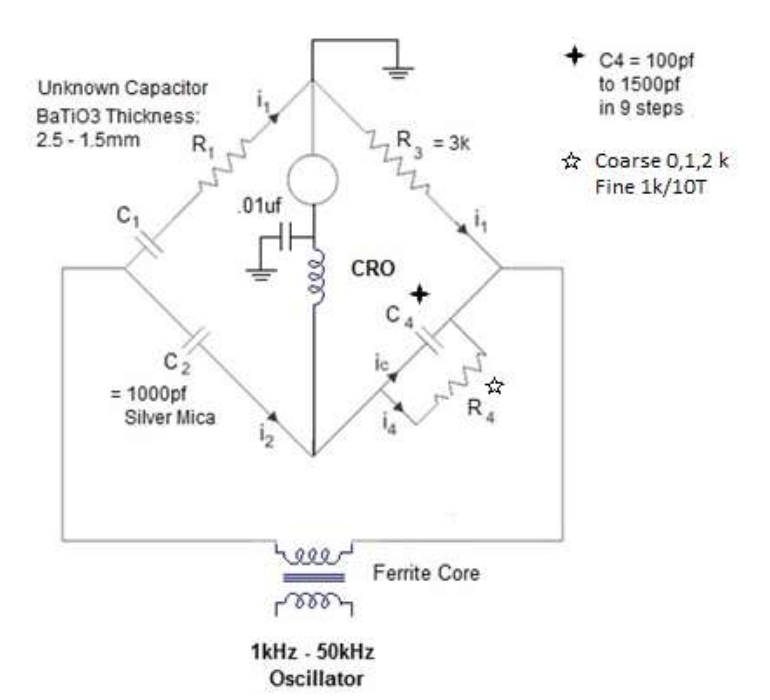
\includegraphics[width=0.7\columnwidth]{images/t5.png}
		\caption{Schering Bridge}
	\end{figure}

	A frequency dependence of dielectric constant. The main unit is used in the setup to measure capacitance at frequencies between 1kHz and 50kHz. A built-in oscillator and a Schering Bridge \hyperref[fig:setup]{Figure 3} are used to accomplish this. Here, the value of the unknown capacitance ($BaTiO_3$) C1 is to be ascertained by using R1 as a series electrical resistance. C2 is a typical 1000 pf silver mica capacitor. C4 is a variable capacitor with Coarse and Fine values. The metal film resistance, R3, is 3.0 k. R4 is a variable resistance with "Coarse" and "Fine" 1k/10T potentiometers in series and parallel to C4, respectively. From the bridge balance condition we get:
	
	$$R_1=\frac{R_3 C_4}{C_2}$$
	and,
	$$ C_1=\frac{R_4 C_2}{R_3}$$
	Here C1 is the unknown capacitor and R1 is the equivalent series resistance reflecting losses. The loss factor (dissipation factor) can	be defined as:
	$$\tan\delta=\frac{\epsilon^{'}}{\epsilon^"}$$
	from setup it can be calculated as:
	$$\tan\delta=\omega C_1r_1 = 2\pi fC_1R_1$$
